% Compile with pdfLaTeX (twice), latexmk -pdf main.tex, or tectonic main.tex.
% All numerical performance results below are manually invented illustrations.
\documentclass[conference]{IEEEtran}
\usepackage[T1]{fontenc}
\usepackage{amsmath,amssymb,booktabs,array,graphicx,tikz,listings,xcolor,url}
\usetikzlibrary{arrows.meta,positioning}
\usepackage[hidelinks]{hyperref}
\setlength{\tabcolsep}{4pt}
\newcommand{\sys}{Dev Privacy Guard}
\newcommand{\illustrative}{\textbf{Illustrative values only; no experiment was run.}}
\newcommand{\email}[1]{{\scriptsize\nolinkurl{#1}}}
\lstset{basicstyle=\ttfamily\scriptsize,breaklines=true,columns=fullflexible,frame=single,captionpos=b,showstringspaces=false}
\title{Dev Privacy Guard: Towards Privacy-Preserving Browser Perception and Reasoning Across Dynamic Web Environments}
\author{
\IEEEauthorblockN{Shreshth Rai}
\IEEEauthorblockA{Department of Applied Mathematics\\Delhi Technological University\\Delhi, India\\\email{shreshthrai_mc24b06_039@dtu.ac.in}}
\and
\IEEEauthorblockN{Aksh Aggarwal}
\IEEEauthorblockA{Department of Computer Science\\Delhi Technological University\\Delhi, India\\\email{akshaggarwal_cse_25a01023@dtu.ac.in}}
\and
\IEEEauthorblockN{Abhinash Chahataray}
\IEEEauthorblockA{Department of Electrical Engineering\\Delhi Technological University\\Delhi, India\\\email{abhinashchahataray_ee_25a15011@dtu.ac.in}}
\and
\IEEEauthorblockN{Himal Garg}
\IEEEauthorblockA{Department of Software Engineering\\Delhi Technological University\\Delhi, India\\\email{himalgarg_se_25b01063@dtu.ac.in}}
\and
\IEEEauthorblockN{Vaatsalya Srivastava}
\IEEEauthorblockA{Delhi Technological University\\Delhi, India\\\email{vaatsalyasrivastava_ee_25a19036@dtu.ac.in}}
\and
\IEEEauthorblockN{Shreya Kailash}
\IEEEauthorblockA{Delhi Technological University\\Delhi, India\\\email{shreyakailash_25bd096@dtu.ac.in}}
}
\begin{document}
\maketitle
\begin{abstract}
Browser agents must interpret interfaces containing personal information while reasoning about navigation, document requirements, and incomplete forms. Sending complete screenshots or page text to a hosted model exposes information that may be unnecessary for planning, whereas indiscriminate masking can remove the structure needed to act correctly. This paper proposes \sys, a supervised architecture that separates browser-local perception and private execution from remote reasoning. The intended system combines DOM and accessibility evidence, lightweight computer vision, optical character recognition, face detection, calibrated redaction, and change-aware local caching. An encrypted vault exposes task-scoped references instead of private values; a guarded executor resolves those references only when entering authorized information into a destination website. Human review is bound to the exact outgoing image, accompanying text, and reasoning provider. A proposed benchmark measures privacy coverage, interface understanding, task completion, resource use, and latency, with automatic detection evaluated separately from manual corrections. \textbf{This is an ideation-stage research draft: no dataset collection, model training, benchmark run, or user study is claimed. All reported performance numbers are manually constructed hypothetical examples, not empirical or simulation results.} An illustrative operating point of 97.1\% detection F1, 99.2\% sensitive-pixel coverage, and 91.0\% task success demonstrates the intended reporting format. The contribution is an explicit system design and testable evaluation protocol for privacy-aware browser assistance.
\end{abstract}
\begin{IEEEkeywords}
Browser agents, local inference, privacy-preserving perception, sensitive-data redaction, visual reasoning, human-in-the-loop systems, reference-based execution.
\end{IEEEkeywords}

\section{Introduction}
Natural-language browser assistance offers a direct way to navigate unfamiliar websites, complete applications, and combine information distributed across documents. A user should be able to specify a goal, provide selected facts, and receive a completed form for review without describing every click. This apparently simple interaction requires several distinct capabilities: identifying the current interface, interpreting field semantics, selecting appropriate information, recovering from validation errors, and recognizing when further authorization is necessary.

The privacy challenge arises because the evidence used for these decisions often contains more information than the decision requires. A bank statement may expose transaction details when only its reporting period is relevant. A screenshot may contain account identifiers, a photograph, an address, and unrelated notifications even when the next action is merely to open an application tab. Removing all text and imagery would avoid some disclosures but also destroy useful evidence about layout, labels, and error messages. The system must therefore minimize unnecessary disclosure while retaining enough context for reliable planning.

The central proposition of \sys\ is that remote reasoning does not ordinarily require direct access to every private value that a browser action uses. The planner can associate an ``Applicant name'' reference with a ``Full name'' field; the actual name can be resolved locally. Similarly, a local decimal tool can compute an authorized total without placing the source transactions in model context. This separation shifts private-value handling into explicit local operations and leaves navigation and semantic interpretation to a hosted language or vision-language model.

Browser task benchmarks such as WebArena and VisualWebArena motivate evaluating completed tasks in realistic, stateful environments rather than judging only plausible action descriptions~\cite{webarena,visualwebarena}. Our proposed evaluation adds a second axis: the information crossing the reasoning boundary. A successful task accompanied by an unapproved disclosure is not a privacy success. Conversely, a blocked task with a completely masked screen is not evidence of useful automation.

The intended contributions are: (1) a browser-local multimodal perception and redaction architecture that combines complementary detectors; (2) a reference-based execution protocol with observation binding, scoped disclosure, and exact-payload approval; (3) a change-aware cache that reuses local computation without treating stale privacy masks as valid; and (4) a reproducible evaluation design that reports task utility, leakage, human intervention, and resource costs together. These are proposed contributions, not claims that the complete architecture has been deployed or experimentally validated.

We assume an uncompromised user device, trusted local companion, and correctly enforced browser isolation. Website content and model-generated actions are untrusted. The hosted provider may retain whatever is sent to it; the architecture therefore attempts to prevent unnecessary input disclosure before transmission. It does not provide differential privacy, cryptographic private inference, or protection from a compromised operating system. The destination website receives authorized filled values, potentially through input event handlers before final submission. Privacy from the reasoning provider and disclosure to the destination website are distinct policies.



\section{Related Works}
WebArena introduces an environment for evaluating autonomous web agents through realistic tasks and execution-based outcomes~\cite{webarena}. Its relevance here is methodological: completion should be checked against resulting website state. Our proposed protocol adds outbound-data inspection and authorization checks to this outcome-based evaluation; it does not borrow or claim improvement over published WebArena scores.

VisualWebArena extends web-agent evaluation to visually grounded tasks~\cite{visualwebarena}. This motivates retaining useful non-sensitive visual structure when DOM information is incomplete. Its evaluation setting does not, by itself, establish the effectiveness of our proposed redaction or reference mechanism. Separate controlled tests are needed to determine how masking changes action selection.

MobileViT combines convolutional and transformer components in a lightweight vision architecture~\cite{mobilevit}. It is a candidate backbone for browser-local UI-region analysis, not a ready-made sensitive-information detector. A task-specific head, suitable data, and browser-runtime validation would be needed before claiming that it recognizes private regions. The proposed design keeps this distinction explicit: semantic region classification can support a privacy decision but cannot replace textual and contextual evidence.

BlazeFace investigates lightweight face detection for mobile GPU inference~\cite{blazeface}. It provides a relevant model family for locating faces that should be masked in outgoing screenshots. Face localization neither identifies an individual nor detects all forms of personal information. The proposed pipeline uses it as one independent source of spatial evidence and avoids biometric identification.

ONNX Runtime Web provides browser inference through JavaScript, including WebAssembly and supported GPU execution providers~\cite{ort}. Operator support and model size constrain deployment. Browser-local execution is consequently treated as a condition to verify with an exported model, rather than inferred from a model's small parameter count. The design includes measured fallbacks and on-demand loading to limit memory pressure.

Indirect prompt injection research shows how attacker-controlled external content can redirect LLM-integrated applications~\cite{injection}. Redaction alone does not solve this problem: an entirely public instruction on a webpage can still be malicious. \sys\ therefore separates webpage evidence from user authority and validates proposed actions against local permissions. The architecture limits consequences through a narrow tool set, reference scoping, and destination checks, while recognizing that semantic manipulation remains a challenge.



\section{Methodology}
\subsection{Overview of the Proposed Approach}
The intended architecture contains a browser extension, a local companion with a review dashboard and encrypted vault, a hosted reasoning endpoint, and a guarded execution adapter. The extension observes the page and runs browser-local perception. The companion coordinates tasks, stores reviewed facts, creates sanitized requests, and validates returned actions. The server interprets only the released context. Figure~\ref{fig:architecture} summarizes these boundaries.

At step $t$, define an observation as
\begin{equation}
 o_t=(D_t,I_t,g_t,v_t,\tau_t),
\end{equation}
where $D_t$ is bounded DOM/accessibility evidence, $I_t$ is the screenshot, $g_t$ contains viewport and coordinate transforms, $v_t$ is the page version, and $\tau_t$ binds the task, tab, and frame. A local sanitizer $S$ creates $z_t=S(o_t,\mathcal{V},\pi)$ using vault knowledge $\mathcal{V}$ and policy $\pi$. The remote planner proposes
\begin{equation}
 a_t=f_{\theta}(q,z_t,\mathcal{R}_t,h_t),
\end{equation}
where $q$ is the sanitized goal, $\mathcal{R}_t$ is the authorized reference catalog, and $h_t$ is sanitized history. Private values are excluded from $\mathcal{R}_t$; it contains identifiers, types, and minimal labels.

The executor applies a local predicate $\operatorname{Allow}(a_t,\tau_t,v_t,\pi)$ before resolving arguments. If the page changed, the origin is unauthorized, or a reference was revoked, the proposal is rejected and the page is re-observed. A successful local action yields sanitized verification evidence for the next step. A missing-information response pauses the same task rather than inventing a value or restarting with broader access.

\begin{figure*}[t]
\centering
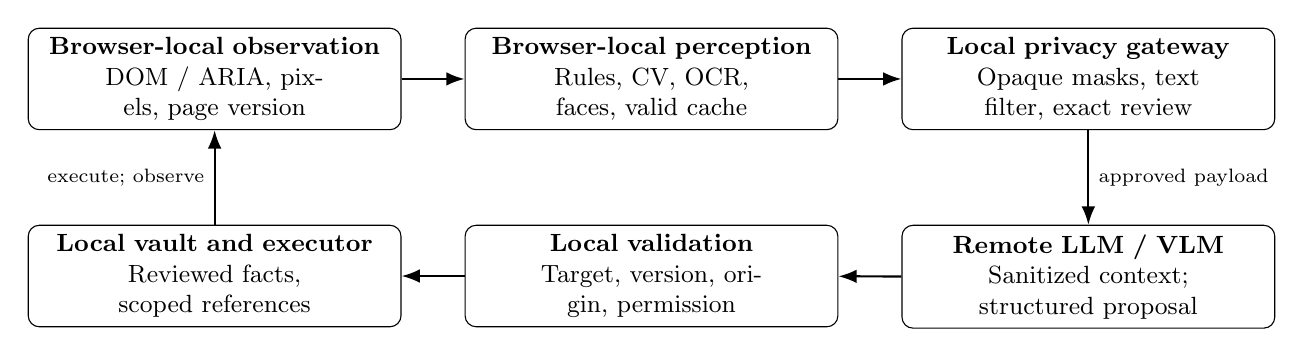
\begin{tikzpicture}[node distance=5mm and 8mm,box/.style={draw,rounded corners,align=center,font=\small,text width=4.5cm,minimum height=1.1cm},arr/.style={-{Latex},thick}]
\node[box] (obs) {\textbf{Browser-local observation}\\DOM / ARIA, pixels, page version};
\node[box,right=of obs] (per) {\textbf{Browser-local perception}\\Rules, CV, OCR, faces, valid cache};
\node[box,right=of per] (rev) {\textbf{Local privacy gateway}\\Opaque masks, text filter, exact review};
\node[box,below=12mm of obs] (vault) {\textbf{Local vault and executor}\\Reviewed facts, scoped references};
\node[box,below=12mm of per] (check) {\textbf{Local validation}\\Target, version, origin, permission};
\node[box,below=12mm of rev] (model) {\textbf{Remote LLM / VLM}\\Sanitized context; structured proposal};
\draw[arr] (obs)--(per); \draw[arr] (per)--(rev); \draw[arr] (rev)--node[right,font=\scriptsize]{approved payload}(model);
\draw[arr] (model)--(check); \draw[arr] (check)--(vault); \draw[arr] (vault)--node[left,font=\scriptsize]{execute; observe}(obs);
\end{tikzpicture}
\caption{Proposed perception--reasoning--execution loop. Original screenshots, private values, and raw visual embeddings remain in local processing. Authorized values entered into a website are disclosed to that website.}
\label{fig:architecture}
\end{figure*}

The system optimizes a constrained utility objective rather than a single accuracy score:
\begin{equation}
 \max U_{\rm task}\quad\text{s.t.}\quad
 L_{\rm disclosure}\leq\epsilon,\ T_{95}\leq B_T,\ M_{\rm peak}\leq B_M.
\end{equation}
Here $\epsilon$ and the resource budgets are evaluation targets, not proven guarantees. A zero-tolerance rule can block recognized credentials, but unknown sensitive content still requires empirical detection assessment. Human review is an additional control, not a mathematical proof of complete sanitization.

\subsection{Dataset Construction}
We propose a benchmark of synthetic and permissioned web pages containing forms, document previews, account dashboards, messages, and mixed visual content. Every example would bind a screenshot and DOM snapshot to sensitive spans, pixel masks, field labels, permitted actions, and expected page state. Synthetic identities avoid using the authors' real contact information as benchmark data. Original documents and ground-truth values would remain local during privacy tests.

\subsubsection{Scenario-Based and Monte Carlo Augmentation}
A base page would be varied through sampled viewport sizes, zoom, scroll positions, theme, font size, field order, image compression, and delayed content insertion. Each transformation must update its annotations. Rendering a name into a canvas, for example, transfers the sensitive region from a DOM span to pixel ground truth. A perturbation that clips a field also changes what is visible and potentially actionable.
\begin{equation}
 \widetilde{o}=A(o;\xi),\qquad \xi\sim p(\xi).
\end{equation}
The generator would save the random seed and transformation manifest. Identity swaps and translated layouts derived from the same base template remain in the same split to prevent leakage. Stress cases include late-loading avatars, autocomplete overlays, cross-origin frames, disappearing controls, and canvas changes without informative DOM mutations. Monte Carlo here describes a proposed sampling procedure; no samples were generated for the numerical examples in this draft.

\subsubsection{Multilingual Q\&A Generation}
Questions would test both interface perception and action reasoning. Closed questions include ``Which field requests the applicant's address?'' and ``Is the document period available?'' Open questions include ``Why should the task pause?'' and ``What additional information is required before continuing?'' English and Hindi are proposed initial annotation languages; broader coverage depends on OCR and reviewer availability.

Answers must be grounded in labeled page state and disclosure policy. A valid answer can be a field identifier, a missing-information request, or a short explanation that cites public labels. It must not contain a hidden reference value. Human reviewers would check whether each question is answerable from the sanitized view, distinguishing impossible cases from model errors. Question paraphrases alone would not count as new independent task families.

\begin{figure}[t]
\centering
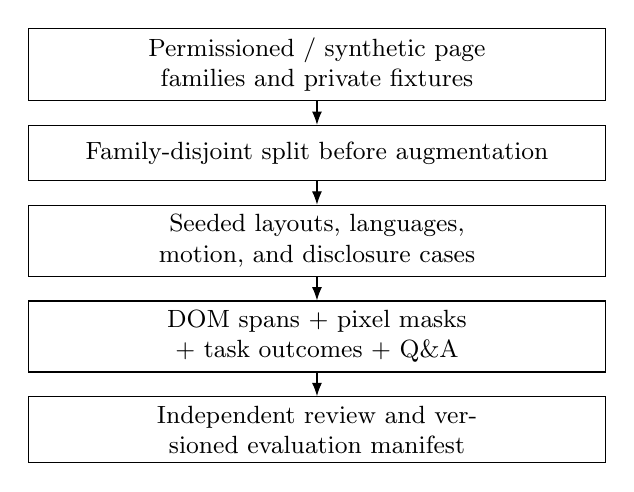
\begin{tikzpicture}[node distance=3mm,box/.style={draw,align=center,text width=7.1cm,font=\small,minimum height=7mm},arr/.style={-{Latex}}]
\node[box] (a) {Permissioned / synthetic page families and private fixtures};
\node[box,below=of a] (b) {Family-disjoint split before augmentation};
\node[box,below=of b] (c) {Seeded layouts, languages, motion, and disclosure cases};
\node[box,below=of c] (d) {DOM spans + pixel masks + task outcomes + Q\&A};
\node[box,below=of d] (e) {Independent review and versioned evaluation manifest};
\draw[arr] (a)--(b);\draw[arr] (b)--(c);\draw[arr] (c)--(d);\draw[arr] (d)--(e);
\end{tikzpicture}
\caption{Proposed dataset construction pipeline. This figure specifies future work; it does not represent a collected dataset.}
\label{fig:data}
\end{figure}

\subsection{Model Architecture}
\textit{Template correspondence: the following five numbered headings retain the supplied audio paper's exact wording. Their content explicitly identifies the browser-agent counterparts; they do not imply that an audio MoE or speaker-identification system is part of this project.}

\subsubsection{Overview of the Mixture-of-Experts Framework}
The browser counterpart is a selectively scheduled set of perception specialists: DOM rules, private-value matching, OCR, UI-region vision, and face detection. This is an orchestration design, not a claim of a trained sparse MoE layer. Each expert produces a common record containing category, region or text span, calibrated confidence, evidence source, detector version, and observation binding.

Cheap DOM rules run first. Password inputs and known private values trigger mandatory masking. OCR is scheduled for image text and otherwise unresolved regions. A MobileViT-style backbone with a suitable task head would propose UI regions, while a lightweight face detector identifies portrait regions~\cite{mobilevit,blazeface}. A face box supports redaction, not recognition. Unsupported areas are conservatively covered or withheld.

Let $u_k(o_t)\in\{0,1\}$ indicate whether specialist $k$ is scheduled. Its findings are combined through a policy union:
\begin{equation}
 \mathcal{B}_t=\operatorname{Merge}\!\left(\bigcup_{k:u_k=1}E_k(o_t)\right).
\end{equation}
Mandatory credential evidence is never averaged away by disagreement from another expert. Detector confidence values require separate calibration; a face score and an OCR score are not interchangeable probabilities. A future learned scheduler could reduce cost, but it must preserve mandatory checks and be compared with deterministic scheduling.

\subsubsection{Multilingual ASR and Speech Embedding Expert}
This retained template label corresponds only to the optional voice task-entry surface. A transcription produces an editable goal; it does not authorize browsing, disclosure, or submission. The principal browser-language pipeline instead uses DOM text and local OCR to recover labels and text from images. Language-aware normalization may help align ``Full name'' with a name reference while preserving the original local text for execution checks.

A fully local speech recognizer is a possible extension. If a hosted transcription service is used, the original audio is disclosed to that service before the transcript can be sanitized. That path must be separately authorized and reported; subsequent text filtering cannot undo the audio disclosure. The proposed browser benchmark disables cloud voice input so that its privacy measurements concern the browser reasoning path. We make no speech recognition accuracy or speech-embedding training claim.

\subsubsection{Speaker Diarization and Identity Encoding}
The relevant browser counterpart is source attribution and reference identity, not speaker diarization. Each confirmed fact has a subject, document source, review status, scope, and version. Two documents may describe different people or reporting periods; matching their field labels does not make their values interchangeable. A task selects explicit references and cannot silently gain access to all vault records.

A record can be represented as
\begin{equation}
 r=(id,type,subject,source,scope,version,value).
\end{equation}
Only an opaque identifier, necessary type, and minimal public label are released to the planner. Subject and provenance metadata are reduced when they themselves disclose private information. Task-local random identifiers prevent meaningful cross-task linkage through predictable reference names. Vault encryption protects stored records; it does not encrypt values after an authorized browser insertion or cover ordinary browser cache files.

Documents are parsed or OCR-processed locally with page, size, and processing limits. Extracted candidates remain unavailable until the user reviews them. Document-specific totals retain their period and source and do not overwrite reusable profile facts. A narrow local calculation tool can combine authorized numeric references using decimal arithmetic, register its result as another reviewed or policy-permitted reference, and return only sanitized status.

\subsubsection{Audio Event and Paralinguistic Experts}
The browser counterparts of this template heading are page-event detection and non-textual visual signals. No audio-event or emotion-recognition component is proposed. Mutation, input, navigation, scroll, and resize events mark regions dirty; screenshot checks detect relevant canvas or image changes. A debounce window coalesces repetitive changes without authorizing reuse of uncertain masks.

A cache entry binds task, origin, frame, region fingerprint, geometry, model version, policy version, and expiry. Reuse requires all applicable bindings to match and the region to remain unchanged. Navigation invalidates page-specific state. Scroll and resize invalidate geometry unless a verified transform can reconstruct it. Periodic full refreshes provide a backstop for changes that do not produce useful DOM events. Raw embeddings remain local because they may encode sensitive content.

For a cached region $j$, the validity predicate is
\begin{equation}
 V_j=\mathbf{1}[b_j=b'_j\land f_j=f'_j\land t<t_{{\rm exp},j}],
\end{equation}
where $b_j$ collects scope and version bindings and $f_j$ is its verified content fingerprint. A cache miss incurs extra work; uncertainty cannot justify a hit. A model call is requested at meaningful decisions, such as a new section, ambiguous layout, validation error, or missing document, rather than on every animation frame.

\subsubsection{Temporal-Semantic Fusion and Reasoning Head}
Fusion aligns text and visual evidence to the same observation and coordinate system. A CSS region is transformed to screenshot pixels using measured viewport scale and offsets; it is not blindly multiplied by device pixel ratio. Frames, browser zoom, cropping, and screenshot resizing must be accounted for. If correspondence cannot be verified, sharing is blocked pending a new observation.

For sensitive regions $\mathcal{B}_t$, the binary mask and released image are
\begin{align}
 M_t(p)&=\mathbf{1}\left[p\in\bigcup_{b\in\mathcal{B}_t}\operatorname{dilate}(b,m_b)\right],\\
 I'_t(p)&=(1-M_t(p))I_t(p)+M_t(p)c,
\end{align}
where $c$ is an opaque replacement color and $m_b$ is a safety margin. High-confidence boxes can use tight margins; ambiguous or uninspectable areas need larger masks or review. Blur is excluded from the outgoing privacy mechanism because it can retain recognizable structure. Pixels and text are sanitized independently: covering a screenshot does not remove the same value from DOM text, URLs, tool output, or history.

The user reviews the exact outgoing screenshot together with text and provider identity. Approval is bound to
\begin{equation}
 h=H(\operatorname{canon}(payload,provider,task,versions)).
\end{equation}
A mask edit changes the artifact and requires a new approval. The gateway sends the approved immutable payload, not a reconstructed screenshot captured later. Review of a screenshot never grants authority to submit a form.

The reasoning head is a hosted LLM/VLM consuming sanitized labels and imagery, not arbitrary local backbone embeddings. Its narrow action schema includes navigation, supported clicks, reference input, questions, and completion proposals. Local validation binds the proposal to a trusted target and checks origin and permission. Unrestricted JavaScript, arbitrary file operations, and unvalidated literal private-value input are excluded. Unexpected instructions in a webpage cannot grant new tool authority~\cite{injection}.

\begin{lstlisting}[caption={Illustrative sanitized observation and action proposal. Values are resolved locally, outside model context.},label={lst:ref}]
{"fields":[{"element_id":"el_12",
 "label":"Full name","state":"empty"}],
 "references":[{"id":"ref_7",
 "type":"person_name","label":"Applicant name"}]}
{"action":"input_ref","element_id":"el_12",
 "value_ref":"ref_7"}
\end{lstlisting}

\begin{figure}[t]
\small
\hrule\vspace{4pt}
\textbf{Algorithm 1: Proposed private browser reasoning loop}
\begin{enumerate}
\item Bind task, tab, frame, origin, page version, and selected references.
\item Capture consistent DOM and pixels; retry if geometry or version is uncertain.
\item Invalidate dirty cache entries; run required local rules and perception specialists.
\item Merge findings; mask pixels; sanitize text, URLs, results, and history.
\item Obtain exact-payload image approval; block denied or changed payloads.
\item Request a structured proposal from the hosted reasoning model.
\item If information is missing, pause for local extraction and fact review; refresh selected references and return to step 2.
\item Validate proposal scope, target, and freshness. Obtain separate consequential-action approval when needed.
\item Resolve permitted references locally, execute, and verify using fresh evidence.
\item Continue within budgets, or stop with a sanitized completion or failure report.
\end{enumerate}
\hrule
\caption{Policy-mediated inference and execution. Locking the vault cancels active work and clears sensitive transient caches.}
\label{fig:algorithm}
\end{figure}

\subsection{Training Strategy and Optimization}
The proposed training program separates perception adaptation from policy enforcement. First, evaluate pretrained components on validation pages and establish rule-based baselines. Second, if UI-region recognition is inadequate, train a small detection head using region annotations. Third, calibrate detector thresholds on validation data, then freeze thresholds before held-out testing. The hosted reasoning model can remain frozen; end-to-end training through the redaction boundary is not required.

A candidate perception objective is
\begin{equation}
 \mathcal{L}=\lambda_c\mathcal{L}_{\rm class}
 +\lambda_b\mathcal{L}_{\rm box}+\lambda_s\mathcal{L}_{\rm sensitive},
\end{equation}
with nonnegative weights tuned on validation data. Box loss concerns localization, class loss concerns UI categories, and sensitive-region loss emphasizes missed private regions. They supervise different outputs and should be reported separately. Policy rules for credentials and approvals remain deterministic even if a learned detector predicts low risk.

A proposed starting recipe is a frozen backbone followed by limited fine-tuning, batch size 16, AdamW with learning rate $10^{-4}$, and at most 30 epochs with validation-based early stopping. These are draft settings, not a completed training configuration. Exported and quantized variants must be reevaluated for privacy recall because deployment optimizations can alter outputs. Model identifiers, weights, licenses, conversion scripts, seeds, and calibration artifacts would be recorded.



\section{Experimental Setup and Evaluation Protocol}
\subsection{Dataset Composition and Preprocessing}
The planned benchmark contains 200 base page families: 50 application-form, 40 account-dashboard, 40 document-preview, 40 messaging, and 30 mixed-media families. Thirty rendered states per family would yield 6,000 screenshots. Four task trajectories per family would yield 800 task definitions. These are proposed collection targets, not existing dataset counts.

A family-disjoint 70/15/15 partition would allocate 140/30/30 families, corresponding to 4,200/900/900 screenshots and 560/120/120 tasks. Augmentations are generated only after assignment. Multi-page trajectories remain within one split, and duplicated identity records or translated templates are checked for unintended linkage. The held-out pages should be independently authored where practical.

Labels cover credentials, names, contact details, addresses, financial identifiers, document numbers, faces, and task-relevant public controls. Overlapping categories require a documented matching rule. Two reviewers would independently annotate a subset, reconcile disagreements, and publish agreement statistics after collection. We do not invent reviewer agreement values. Screenshots retain capture metadata; original-resolution masks remain the ground truth even when model input is resized.

\subsection{Baseline Models for Comparison}
Five controlled configurations are proposed. B0 sends raw screenshots and page text and serves only as a synthetic-data utility ceiling. B1 uses DOM and pattern redaction. B2 additionally runs OCR and face detection over each observation without change-aware reuse. B3 masks the entire image while retaining sanitized text. DPG-A combines multimodal redaction with validated caching. DPG-R adds user review to DPG-A and is evaluated separately.

These are defined experimental configurations, not named commercial systems or published benchmark results. All share the same hosted model snapshot, task instructions, permitted action set, budgets, and website fixtures. Only the intended privacy and perception components differ. Final-action approval policy is kept constant across conditions. A raw-input baseline must use exclusively synthetic or appropriately authorized fixtures.

Manual screenshot correction is disabled for automatic detector scoring. For the separate reviewed condition, record reviewer time, number of mask additions, denials, and remaining leakage. A reviewed score cannot be credited to the automatic model. Repeated trials use paired task seeds and restore website state to avoid differences caused by previous actions.

\subsection{Evaluation Metrics}
Sensitive-region detection uses precision $P$, recall $R$, and F1 with category-compatible one-to-one matching at a predeclared IoU threshold of 0.5:
\begin{equation}
 P=\frac{TP}{TP+FP},\quad R=\frac{TP}{TP+FN},\quad F_1=\frac{2PR}{P+R}.
\end{equation}
Report micro and per-category scores; macro F1 is computed from per-category F1 values rather than inferred from pooled precision and recall. Empty-category cases require an explicit convention.

Let $G_i$ be sensitive ground-truth pixels, $M_i$ the emitted mask, and $\Omega_i$ the screenshot. Coverage and non-sensitive over-masking are
\begin{align}
 C&=\frac{\sum_i|G_i\cap M_i|}{\sum_i|G_i|},\\
 O&=\frac{\sum_i|M_i\setminus G_i|}{\sum_i|\Omega_i\setminus G_i|}.
\end{align}
Mask IoU is also reported, but small highly sensitive regions must not disappear behind a favorable aggregate area score. Outbound tests count seeded secrets appearing in actual requests, including retries and history. Define exposure rate as requests containing at least one seeded secret divided by inspected requests, and separately report catastrophic credential/face leaks. Text and image inspection have different failure modes and require separate checks.

Task success is verified against fixture state. Policy-compliant success additionally requires no unapproved consequential action or detected prohibited reasoning disclosure. Field identification accuracy and Q\&A accuracy use held-out labels. All task results include exact numerators and denominators when measured; illustrative percentages in this draft have no trial counts behind them.

Resource measurement includes cold and warm latency, p50/p95 stage timings, peak incremental process memory, CPU utilization, available GPU profiling, model download size, and cache hit rate. Human approval time is reported separately and included in total task duration:
\begin{equation}
 T_{\rm total}=T_{\rm local}+T_{\rm network/model}+T_{\rm execution}+T_{\rm human}.
\end{equation}
P95 values of individual stages must not simply be added to estimate total p95. Instrument the complete trajectory directly. Missing GPU telemetry is reported as unavailable, not zero.

\subsection{Implementation Details}
The target implementation uses a Chrome extension for DOM/accessibility observation and browser-local model inference, a Python companion for orchestration and local document processing, and a dashboard for vault and screenshot review. Browser Use is an automation foundation behind product-owned observation and execution adapters. AES-GCM-encrypted records in local SQLite would be unlocked with a passphrase-derived key; reference resolution occurs only inside the trusted execution path.

ONNX Runtime Web with a compatible WebGPU model is the preferred candidate path, with measured WebAssembly fallback~\cite{ort}. No specific MobileViT export or complete vision stack is assumed to work without operator and memory validation. A proposed initial device is an M1 MacBook Air with 8 GB RAM, one active task, and a bounded worker count. Suggested initial limits are a 1,024-pixel perception long edge, 128 MiB cache, 200 ms event debounce, 30-second region expiry, and 40 action steps. They are engineering starting points, not optimal measured settings.

The benchmark would pin browser, OS, detector, runtime, and hosted model versions. Network condition, screen scale, cold-start policy, and prompt version would be recorded. Local telemetry stores timings and counts without private payloads. For privacy auditing, synthetic request fixtures can be retained in a separate controlled harness. A reproducibility release should include generators, labels, hashes, configurations, and scoring code before making empirical performance claims.

\section{Results and Discussion}
\textbf{Status of this section.} All table entries and numerical improvements below are manually invented to demonstrate a possible research-paper presentation. They are neither measured outcomes nor outputs of a simulator, and they establish no superiority, confidence interval, or statistical significance. Dataset sizes in Section IV are planned targets. The discussion explains what such observations would mean if later reproduced.

\subsection{Quantitative Evaluation}
Table~\ref{tab:main} presents one hypothetical privacy--utility trade-off. DPG-A is assigned 97.1\% micro F1, 99.2\% pixel coverage, and 91.0\% task success. The raw-input condition has higher hypothetical task success but no redaction coverage. Full-image masking covers every sensitive pixel while also masking every non-sensitive pixel; its reduced hypothetical task success illustrates why privacy coverage alone is insufficient.

\begin{table*}[t]
\centering\small
\caption{Hypothetical operating points for defined configurations. \illustrative\ F1 is micro-averaged region detection; coverage and over-mask concern image pixels; latency is warm local processing per observation.}
\label{tab:main}
\begin{tabular}{lrrrrrr}
\toprule
Configuration & Detection F1 (\%) & Coverage (\%) & Over-mask (\%) & Task success (\%) & p50 (ms) & p95 (ms)\\
\midrule
B0: Raw context & -- & 0.0 & 0.0 & 94.0 & 25 & 60\\
B1: DOM + patterns & 86.4 & 88.2 & 3.1 & 89.0 & 40 & 85\\
B2: Multimodal, no cache & 97.1 & 99.2 & 7.4 & 91.0 & 180 & 360\\
B3: Full-image mask & -- & 100.0 & 100.0 & 70.0 & 32 & 70\\
DPG-A: Multimodal + cache & 97.1 & 99.2 & 7.4 & 91.0 & 110 & 240\\
DPG-R: DPG-A + review & -- & 99.8 & 8.6 & 92.0 & -- & --\\
\bottomrule
\end{tabular}
\end{table*}

The hypothetical B2 and DPG-A detection values are deliberately equal: cache reuse is intended to preserve outputs when valid while reducing redundant computation. Equality here is a design hypothesis, not a finding. DPG-R has no automatic F1 entry because manual additions would confound attribution. Its latency is omitted from that table because review introduces a separately measured human-time distribution.

\subsubsection{Metric-specific Insights.}
A constructed precision of 96.8\% and recall of 97.4\% produce approximately 97.1\% F1. High pixel coverage can coexist with lower region recall because missed regions may occupy few pixels. A missed short credential is nevertheless severe. For this reason, a future evaluation must publish category-specific false negatives and actual outbound exposures alongside pixel coverage.

The invented 110 ms versus 180 ms p50 values imply
\begin{equation}
 \Delta_{\rm latency}=\frac{180-110}{180}\times100\%=38.9\%.
\end{equation}
This arithmetic is a calculation from invented inputs, not measured acceleration. It concerns local warm processing, not total task time, cold starts, or human review. Likewise, 91.0\% versus 89.0\% task success is a two-percentage-point illustrative difference; it is not evidence of a statistically reliable gain.

\begin{table}[t]
\centering\small
\caption{Invented resource and interaction examples for DPG-A. \illustrative\ CPU/GPU and cold-start values would require device-specific profiling.}
\label{tab:resource}
\begin{tabular}{lr}
\toprule
Quantity & Hypothetical value\\
\midrule
Peak incremental local memory & 620 MiB\\
Valid region-cache hit rate & 64.0\%\\
Mean reasoning calls / task, uncached policy & 18\\
Mean reasoning calls / task, event policy & 11\\
Warm local latency p50 / p95 & 110 / 240 ms\\
WASM fallback local p50 / p95 & 340 / 710 ms\\
Median added screenshot-review time / task & 24 s\\
\bottomrule
\end{tabular}
\end{table}

Table~\ref{tab:resource} separates local computation reuse from remote-call scheduling. A cache hit does not automatically eliminate a reasoning call; a meaningful validation error may still require a fresh decision. The invented change from 18 to 11 calls corresponds to 38.9\% fewer calls, independently of the latency example. Neither token cost nor total speedup follows without observing payload size, provider latency, and user waiting time.

\subsection{Ablation Analysis}
The proposed ablations isolate OCR, faces, private-value matching, and caching while keeping the reasoning model fixed. Table~\ref{tab:ablation} gives hypothetical outputs that illustrate the intended reporting structure. Removing OCR is expected to expose image-rendered text; removing face detection is expected to affect portraits; removing known-value matching should particularly affect uncommon identifiers. These expectations require direct category-level evaluation.

\begin{table}[t]
\centering\small
\caption{Manually constructed ablation examples, not experimental findings. Coverage is sensitive-pixel coverage.}
\label{tab:ablation}
\begin{tabular}{lrrr}
\toprule
Configuration & F1 (\%) & Coverage (\%) & p50 (ms)\\
\midrule
Full automatic design & 97.1 & 99.2 & 110\\
Without OCR & 90.2 & 92.5 & 78\\
Without face detector & 93.4 & 94.8 & 96\\
Without known-value match & 94.0 & 96.7 & 106\\
Without cache reuse & 97.1 & 99.2 & 180\\
Without geometry checks & 92.0 & 93.1 & 101\\
\bottomrule
\end{tabular}
\end{table}

Disabling geometry checks is an unsafe stress-test condition permitted only on synthetic fixtures. It asks whether shifted masks expose values after scrolling or resizing. It should never become an optimization option for private browsing. A second cache stress test would deliberately change a cached canvas region and confirm invalidation. Lower latency is useful only when privacy and action bindings remain correct.

Future comparisons should use paired task-family resampling, exact denominators, and confidence intervals. No statistical significance is claimed without trials.

\subsection{Qualitative Analysis and Interpretability}
Consider a hypothetical application workflow. The user selects reviewed name, email, and phone references and asks the agent to reach the final review page. The observer identifies public labels and masks existing private content. After screenshot approval, the planner proposes reference-based input. The executor verifies target and origin, fills the actual values locally, and redacts them in subsequent observations.

The next page requests an address and statement total. Rather than deriving these from an unrelated record, the planner returns a missing-information request. The user uploads a synthetic statement; local extraction produces candidates with source and period. The user confirms them, chooses task scope, and resumes with selected new references. A fresh observation accounts for any website changes during the pause. A decimal total is calculated locally if permitted. The task stops at the completed review page until separate submission authorization is given.

Interpretability is supplied by evidence and action records: which detector produced a mask, which observation an action targeted, which reference type was used, why execution was blocked, and which payload was approved. Concise decision explanations and observable tool traces are sufficient; access to a model's hidden internal reasoning is not assumed. Reference values and original screenshots should not be copied into ordinary audit logs.

Failure cases include uncommon private strings that evade rules, tiny OCR text, obscured faces, rapid content replacement, and a public label whose meaning depends on hidden context. Over-masking may hide a validation message, while under-masking may expose a private value beside it. A user can deny sharing, add masks, clarify the task, or take over manually. Such interventions must be counted rather than removed from the benchmark as inconvenient examples.

\subsection{Discussion}
The architecture is intended to make disclosure a controlled dataflow property. Every model request, retry, tool result, and history message must cross the same gateway. A single unrestricted fallback path can defeat the design even if the main screenshot filter performs well. Future verification must therefore inspect transport behavior and failure recovery in addition to detector accuracy.

There is a fundamental utility trade-off when an authorized decision genuinely depends on a private value. Reference labels are enough for routine field placement but may be insufficient for comparing eligibility rules against detailed records. Narrow local tools can perform defined computations; unsupported reasoning must be escalated to the user or handled by an explicitly authorized local capability. Sending hidden embeddings to the server is not an established privacy-preserving shortcut.

Human review introduces workload and possible habituation. The proposed system requires exact screenshot approval because this makes the released artifact inspectable, yet users can still miss small disclosures. The reviewed condition therefore needs its own study of time, error, and comprehension. An illustrative 99.8\% coverage score would still leave residual exposed pixels and would not justify a ``zero leakage'' claim.

Several deployment questions remain open: browser operator compatibility, memory pressure on low-resource devices, reliable coordinate mapping, multilingual OCR, inaccessible frames, authentication flows, and recovery after uncertain website actions. Login, OTP, CAPTCHA, and unsupported custom controls may require manual takeover. A crash must not replay a consequential action whose outcome is uncertain. Locking the vault revokes access and clears transient state; subsequent work requires a fresh observation and authorization checks.



\section*{Conclusion}
This paper proposed \sys, a browser-agent architecture that keeps sensitive perception and private-value execution local while using hosted reasoning over sanitized context. Its central mechanisms are complementary browser-local detectors, independent text and pixel sanitization, geometry-bound observations, exact-payload image approval, scoped private references, and guarded execution. Change-aware caching is designed to reduce redundant local computation without reusing uncertain privacy state, while reviewed document intake supports missing-information requests within the same task.

The draft defines a dataset construction plan, baseline configurations, privacy and utility metrics, and ablations suitable for evaluating the intended approach. All numerical performance values are illustrative inventions; no empirical validation is claimed. Future work must establish browser-compatible model artifacts, calibrate detectors, collect independent ground truth, exercise dynamic-page failures, inspect actual outbound requests, and measure human review costs. The intended research outcome is a reproducible account of when useful browser reasoning can operate with reduced disclosure, together with clear evidence of where that separation fails.

\begin{thebibliography}{9}
\bibitem{webarena} S. Zhou et al., ``WebArena: A realistic web environment for building autonomous agents,'' arXiv:2307.13854, 2023. [Online]. Available: \url{https://arxiv.org/abs/2307.13854}
\bibitem{visualwebarena} J. Y. Koh et al., ``VisualWebArena: Evaluating multimodal agents on realistic visual web tasks,'' arXiv:2401.13649, 2024. [Online]. Available: \url{https://arxiv.org/abs/2401.13649}
\bibitem{mobilevit} S. Mehta and M. Rastegari, ``MobileViT: Light-weight, general-purpose, and mobile-friendly vision transformer,'' arXiv:2110.02178, 2021. [Online]. Available: \url{https://arxiv.org/abs/2110.02178}
\bibitem{blazeface} V. Bazarevsky et al., ``BlazeFace: Sub-millisecond neural face detection on mobile GPUs,'' arXiv:1907.05047, 2019. [Online]. Available: \url{https://arxiv.org/abs/1907.05047}
\bibitem{ort} ONNX Runtime contributors, ``How to add machine learning to your web application with ONNX Runtime,'' documentation, accessed Sep. 11, 2026. [Online]. Available: \url{https://onnxruntime.ai/docs/tutorials/web/}
\bibitem{injection} K. Greshake et al., ``Not what you've signed up for: Compromising real-world LLM-integrated applications with indirect prompt injection,'' arXiv:2302.12173, 2023. [Online]. Available: \url{https://arxiv.org/abs/2302.12173}
\end{thebibliography}
\end{document}
